%% Example data sheet
%% Feel free to modify and use this file for any purpose, under
%% either the LaTeX Project Public License or under public domain.

% Options here are passed to the article class.
% Most common options: 10pt, 11pt, 12pt
\documentclass[10pt]{datasheet}

% Input encoding and typographical rules for English language
\usepackage[utf8]{inputenc}
\usepackage[english]{babel}
\usepackage[english]{isodate}

% tikz is used to draw images in this example, but you can
% also use \includegraphics{}.
\usepackage{tikz}
\usepackage{pgfplots}
\usepackage{circuitikz}
\usetikzlibrary{calc}

% These define global texts that are used in headers and titles.
\title{Low energy semiconductor gas sensor}
\author{Struggle DVC}
\date{November 2024}
\revision{Revision 1}
\companylogo{\Huge $\nabla$ Struggle DVC}

\begin{document}
\maketitle

\section{Features}

\begin{itemize}
\item{High sensitivity to a wide range of gases}
\item{State-of-the-art nanoparticles technology}
\item{Conditioner is not integrated in the package : power efficiency can be optimized to the application}
\item{Long lifetime}
\item{Short to instance response-time}
\item{Environmentally safe}
\item{Low cost at high volume}
\end{itemize}

\section{Description}
The AIME GASNP-2024 is a high-sensitivity gas sensor based on WO3 nanoparticules designed to detect oxydable-gases in the air such as ethanol or ammonia.

It features a sensitive layer of nanoparticles deposited on interdigitated aluminuim combs on a doped silicon substrate. A polysilicon heating element ensures thermal control of the sensing area.

\section{Pins configuration}


\begin{figure}[htbp]
    \centering
    \includegraphics[width=0.25\textwidth]{Pinout.png}
    \centering
    \caption{\centering Sensor Pin Layout}
    \label{fig:enter-label}
\end{figure}

\begin{figure}
    \centering
    \includegraphics[width=0.5\linewidth]{Sensor.png}
    \caption{\centering Gas Sensor AIME}
    \label{fig:enter-label}
\end{figure}

\begin{table}[htbp]
    \centering
    \begin{tabular}{|c|c|}
        \hline
        Pin number & Function \\
        \hline
        1-6 & Temperature sensor (Aluminum resistor) \\
        \hline
        2-4 & Gas sensor \#1 \\
        \hline
        3-8 & Thermal resistor (Polysilicon resistor) \\
        \hline
        7-9 & Gas sensor \#2 \\
        \hline
        5 & NC \\
        \hline
        10 & NC \\
        \hline
    \end{tabular}
\end{table}


\section*{GENERAL CHARACTERISTICS}

% Tableau principal
\begin{table}[h!]
    \centering
    \renewcommand{\arraystretch}{1.1} % Réduit l'espacement entre les lignes du tableau
    \setlength{\tabcolsep}{6pt} % Réduction de l'espacement entre les colonnes
    \small % Réduction de la taille du texte
    \begin{tabular}{|p{5cm}|p{10cm}|}
        \hline
        \textbf{Type} & Chemical sensor \\
        \hline
        \textbf{Materials} & 
        \begin{itemize}
            \item Silicon
            \item N-doped poly-silicon (heater)
            \item Aluminum (temperature measurements)
            \item Nanoparticles of Tungsten Trioxide (WO\textsubscript{3})
        \end{itemize} \\
        \hline
        \textbf{Sensor Type} & Active (power supply required) \\
        \hline
        \textbf{Gas Measurement} & Resistive measure \\
        \hline
        \textbf{Temperature Measurement} & Resistive measure \\
        \hline
        \textbf{Detectable Gases} & 
        \begin{itemize}
            \item Alcohols (-OH)
            \item Ammonia (NH\textsubscript{3})
            \item Carbon Monoxide (CO)
            \item Dihydrogen (H\textsubscript{2})
            \item Ethanol (C\textsubscript{2}H\textsubscript{6}O)
            \item Hydrogen Sulfide (SO\textsubscript{2})
            \item Methane (CH\textsubscript{4})
            \item Nitrogen Dioxide (NO\textsubscript{2})
        \end{itemize} \\
        \hline
        \textbf{Typical Detection Range} & \(> 1 \, {ppm}\) \\
        \hline
        \textbf{Package} & TO-5-10 (10 pins) \\
        \hline
        \textbf{Head Diameter} & 9.5 mm \\
        \hline
        \textbf{Head Height} & 4.7 mm \\
        \hline
        \textbf{Package Height} & 25 mm \\
        \hline
        \textbf{Pin Diameter} & 0.6 mm \\
        \hline
        \textbf{Mounting} & Through hole fixed (THT) \\
        \hline
    \end{tabular}
\end{table}

\section*{GAS SENSOR CHARACTERISTICS}

\makebox[\textwidth][c]{
    \begin{minipage}{0.45\textwidth}
        \centering
        \includegraphics[width=\linewidth]{ethanol.png}
        \captionof{figure}{\centering Gas Sensor exposed to ethanol}
        \label{fig:ethanol}
    \end{minipage}
    \hspace{0.05\textwidth} % Small spacing between images
    \begin{minipage}{0.45\textwidth}
        \centering
        \includegraphics[width=\linewidth]{amoniac.png}
        \captionof{figure}{\centering Gas Sensor exposed to ammoniac}
        \label{fig:enter-label}
    \end{minipage}
}



\clearpage


\section*{ELECTRICAL CHARACTERISTICS}

\begin{table}[h!]
    \centering
    \renewcommand{\arraystretch}{1.5} % Espacement entre les lignes
    \setlength{\tabcolsep}{8pt} % Espacement entre les colonnes
    \makebox[\textwidth]{ % Assure le centrage du tableau
        \begin{tabular}{|c|l|c|c|c|c|}
            \hline
            \textbf{} & \textbf{} & \textbf{Units} & \textbf{Min} & \textbf{Typical} & \textbf{Max} \\
            \hline
            \multirow{3}{*}{\textbf{Resistance}} & Gas Sensor & G$\Omega$ & 0.01 & 1 & 100 \\
            \cline{2-6}
            & Temperature Sensor & $\Omega$ & 57 & 65 & - \\
            \cline{2-6}
            & Heater & $\Omega$ & 70 & 85 & - \\
            \hline
            \multirow{3}{*}{\textbf{Voltage}} & Gas Sensor & V & - & 3.3 & - \\
            \cline{2-6}
            & Temperature Sensor & V & 3.3 & 5 & - \\
            \cline{2-6}
            & Heater & V & 10 & 15 & 20 \\
            \hline
        \end{tabular}
    }
\end{table}

\vspace{1cm}

\makebox[\textwidth][c]{
    \begin{minipage}{0.45\textwidth}
        \centering
        \includegraphics[width=\linewidth]{R_POLY.jpg}
        \captionof{figure}{\centering Characteristics of the Poly-silicon resistor}
        \label{fig:R_POLY}
    \end{minipage}
    \hspace{0.05\textwidth} % Small spacing between images
    \begin{minipage}{0.45\textwidth}
        \centering
        \includegraphics[width=\linewidth]{R_ALU.jpg}
        \captionof{figure}{\centering Characteristics of the Aluminium resistor}
        \label{fig:R_ALU}
    \end{minipage}
}



\clearpage
\onecolumn

\section*{CONFIGURATION}

\begin{figure}[h!]
    \centering
    % Première image
    \begin{subfigure}[b]{1\textwidth}  % Change la largeur à 100% de la ligne
        \centering
        \includegraphics[width=\textwidth]{Configuration.png}  % L'image occupe toute la largeur
        \caption{\centering Package Configuration}  % Sous-titre pour la première image
        \label{fig:config1}
    \end{subfigure}
\end{figure}


\section*{Application}

\begin{figure}[h!]
\centering
\includegraphics[width=0.8\linewidth]{graph.png}
\caption{\centering Application example}
\label{fig:enter-label}
\end{figure}

The resistance of the sensor has a magnitude of Giga Ohm. This means that a voltage divider is not efficient to measure the voltage. The figure above shows the circuit that uses an operational amplifier with a low offset voltage. Therefore, it is not possible to convert the current of the sensor into its resistance using the following formula:

\[
R_{\text{sensor}} = \left(1 + \frac{R_3}{R_2}\right) \cdot R_1 \cdot \frac{V_{cc}}{V_{adc}} - R_1 - R_5
\]

\end{document}



% Switch to next column
\vfill\break

\begin{figure}[h]
    \begin{circuitikz}[european]
        \node[op amp] (amp1) {};
        \node[op amp, below = 0.5cm, xscale = -1] (amp2) {};
        \draw (amp1.out) |- (amp2.-);
        \draw (amp2.-) ++(0, 0.3cm) node[circ]{} to +(2,0) node[above left]{5};
        \draw (amp2.out) to (amp1.+);
        \draw (amp1.+) ++(0, -0.3cm) node[circ]{} to +(-2,0) node[above right]{2};
        \draw (amp1.-) to +(-2,0) node[above right]{1};
        \draw (amp2.+) to +(2,0) node[above left]{4};
        \draw (amp1.out) +(0,0.5cm) node (Vdd) {$\mathrm{V_{DD}}$};
        \draw (Vdd.east) to +(1.5,0) node [above left]{6};
        \draw (amp2.out) +(0,-0.5cm) node (Vss) {$\mathrm{V_{SS}}$};
        \draw (Vss.west) to +(-1.6,0) node [above right]{3};
        \draw ($(amp1.north west) + (-0.5,0.5)$) rectangle ($(amp2.south west) + (0.5,-0.5)$);
    \end{circuitikz}
    \caption{Pinout and internal circuit}
\end{figure}


\begin{figure}[h]
    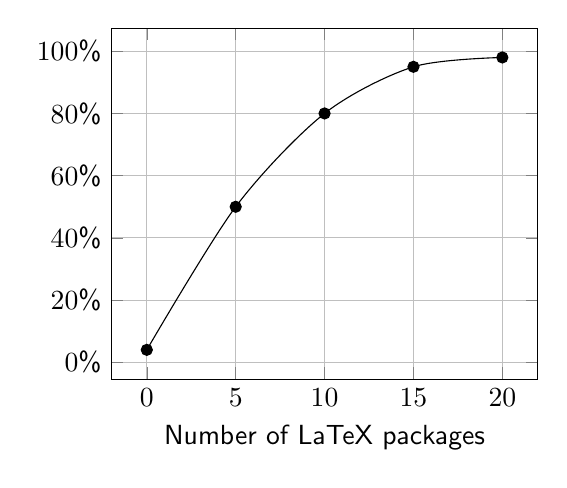
\begin{tikzpicture}
        \sffamily
        \begin{axis}[
            width=7cm,
            xlabel={Number of LaTeX packages},
            ytick distance=20,
            yticklabel={\pgfmathprintnumber{\tick}\%},
            xmajorgrids, ymajorgrids]
        \addplot[smooth,mark=*] plot coordinates {
            (0,4)
            (5,50)
            (10,80)
            (15,95)
            (20,98)
        };
        \end{axis}
    \end{tikzpicture}
    \caption{Typical data sheet production efficiency}
\end{figure}

% For wide tables, a single column layout is better. It can be switched
% page-by-page.
\onecolumn

\section{Electrical Specifications}
All specifications are in $-40\degree C \leq T_A \leq 85\degree C$ unless otherwise noted.

\begin{table}[h]
\begin{threeparttable}
\caption{Example Data Sheet Specifications}
\begin{tabularx}{\textwidth}{l | c | c c c | c | X}
    \thickhline
    \textbf{Parameter} & \textbf{Symbol} & \textbf{Min.} & \textbf{Typ.} & \textbf{Max.} &
    \textbf{Unit} & \textbf{Conditions} \\
    \hline
    Page width  & $p_w$ & 20.9 & 21.0 & 21.1 & cm & \multirow{2}{*}{Standard A4 paper} \\
    Page height & $p_h$ & 29.6 & 29.7 & 29.8 & cm &  \\
    \hline
    Insulation voltage & $E_{max}$\tnote{1} & & 1 & & kV & \\
    \thickhline
\end{tabularx}
\begin{tablenotes}
\item[1]{Based on characterization data, not tested in production.}
\end{tablenotes}
\end{threeparttable}
\end{table}

\section{Absolute Maximum Ratings}

\begin{table}[h]
\caption{Absolute Maximum Ratings of Example Data Sheet}
\begin{tabularx}{\textwidth}{l | X}
    \thickhline
    \textbf{Parameter} & \textbf{Rating} \hspace{5cm} \\
    \hline
    Daily exposure to LaTeX & 24 hours \\
    \thickhline
\end{tabularx}
\end{table}

\textbf{Note:} Stresses above those listed under Absolute Maximum Ratings can
cause permanent damage to the device. This is a stress rating only. Functional
operation of the device is not implied in any conditions above those indicated
in the Electrical Specifications section.

\end{document}


